\documentclass{chi-ext}
% Please be sure that you have the dependencies (i.e., additional LaTeX packages) to compile this example.
% See http://personales.upv.es/luileito/chiext/

%% EXAMPLE BEGIN -- HOW TO OVERRIDE THE DEFAULT COPYRIGHT STRIP -- (July 22, 2013 - Paul Baumann)
% \copyrightinfo{Permission to make digital or hard copies of all or part of this work for personal or classroom use is granted without fee provided that copies are not made or distributed for profit or commercial advantage and that copies bear this notice and the full citation on the first page. Copyrights for components of this work owned by others than ACM must be honored. Abstracting with credit is permitted. To copy otherwise, or republish, to post on servers or to redistribute to lists, requires prior specific permission and/or a fee. Request permissions from permissions@acm.org. \\
% {\emph{CHI'14}}, April 26--May 1, 2014, Toronto, Canada. \\
% Copyright \copyright~2014 ACM ISBN/14/04...\$15.00. \\
% DOI string from ACM form confirmation}
%% EXAMPLE END -- HOW TO OVERRIDE THE DEFAULT COPYRIGHT STRIP -- (July 22, 2013 - Paul Baumann)

\title{Gesture Typing on Virtual Tabletop: Effect of Input on Performance}

\numberofauthors{4}
% Notice how author names are alternately typesetted to appear ordered in 2-column format;
% i.e., the first 4 autors on the first column and the other 4 auhors on the second column.
% Actually, it's up to you to strictly adhere to this author notation.
\author{
  \alignauthor{
    \textbf{Antoine Loriette}\\
    \affaddr{AuthorCo, Inc.}\\
    \affaddr{123 Author Ave.}\\
    \affaddr{Authortown, PA 54321 USA}\\
    \email{antoine.loriette@gmail.com}
  }\alignauthor{
    \textbf{Sebastian Stein}\\
    \affaddr{AuthorCo, Inc.}\\
    \affaddr{123 Author Ave.}\\
    \affaddr{Authortown, PA 54321 USA}\\
    \email{author5@anotherco.com}
  }
  \vfil
  \alignauthor{
    \textbf{Roderick Murray-Smith}\\
    \affaddr{AuthorCo, Inc.}\\
    \affaddr{123 Author Ave.}\\
    \affaddr{Authortown, PA 54321 USA}\\
    \email{author2@anotherco.com}
  }\alignauthor{
    \textbf{John H. Williamson}\\
    \affaddr{AuthorCo, Inc.}\\
    \affaddr{123 Author Ave.}\\
    \affaddr{Authortown, PA 54321 USA}\\
    \email{author6@anotherco.com}
  }
\vfil
}

% Paper metadata (use plain text, for PDF inclusion and later re-using, if desired)
\def\plaintitle{Gesture Typing on Virtual Surfaces: Effect of Input on Performance}
\def\plainauthor{Name}
\def\plainkeywords{Gesture Input, Gesture Keyboard, Mobile, Continuous Interaction, Tabletop, Text Input}
\def\plaingeneralterms{Documentation, Standardization}

\hypersetup{
  % Your metadata go here
  pdftitle={\plaintitle},
  pdfauthor={\plainauthor},
  pdfkeywords={\plainkeywords},
  pdfsubject={\plaingeneralterms},
  % Quick access to color overriding:
  %citecolor=black,
  %linkcolor=black,
  %menucolor=black,
  %urlcolor=black,
}

\usepackage{graphicx}   % for EPS use the graphics package instead
\usepackage{balance}    % useful for balancing the last columns
\usepackage{bibspacing} % save vertical space in references

\usepackage{subfigure}

% own command
\newcommand{\reffigure}[1]{Figure~\ref{#1}}
\newcommand{\reftable}[1]{Table~\ref{#1}}
\newcommand{\smit}[1]{{\small\textit{{#1}}}}
\newcommand{\cdt}[1]{{\small\uppercase{{#1}}}}
\newcommand{\wpm}{\cdt{wpm} }


\begin{document}

\maketitle

\begin{abstract}
The association of tabletop interaction with gesture typing presents potential for physically impaired users. In this work, we use depth cameras to create touch surfaces on regular tabletops. We describe our prototype system and report on a supervised learning approach to fingertips touch classification. We follow with a gesture typing study that compares our system with a control tablet scenario and explore the influence of input size and aspect ratio of the virtual surface on the text input performance. We show that novice users perform with the same error rate at half the input rate with our system as compared to the control condition, that an input size between A5 and A4 present the best tradeoff between precision, performance and user preference and that user's indirect tracking ability seems to be the overall performance limiting factor.

\textcolor{red}{potential for more space}

\end{abstract}

\keywords{\plainkeywords}
% \textcolor{red}{Optional section to be included in your final version.}

\category{H.5.m}{Information interfaces and presentation (e.g., HCI)}{Miscellaneous}.
%See \cite{ACMCCS}
% See: \url{http://www.acm.org/about/class/1998/}
% for help using the ACM Classification system.
% \textcolor{red}{Optional section to be included in your final version, but strongly encouraged.}


% =============================================================================
\section{Introduction}
% =============================================================================
The combination of indirect optically tracked input and potentially projected display (“virtual surfaces”) has several interesting properties. Virtual surfaces, as opposed to touch screens, are well suited to tackle the palm rejection problem and the occlusion problem, offer a choice of size, aspect ratio and texture of the input space and allow interactions with dirty or wet hands.


Depth cameras~\cite{Harrison2011,Xiao2016} have usually been employed to create such surfaces, even though touch classification remains problematic and few systems are available for all camera types. Other work have tried to combine different sensor sources (cite Ubitouch) or other techniques (FTIR?).

\marginpar{
\begin{figure}
    \begin{center}
        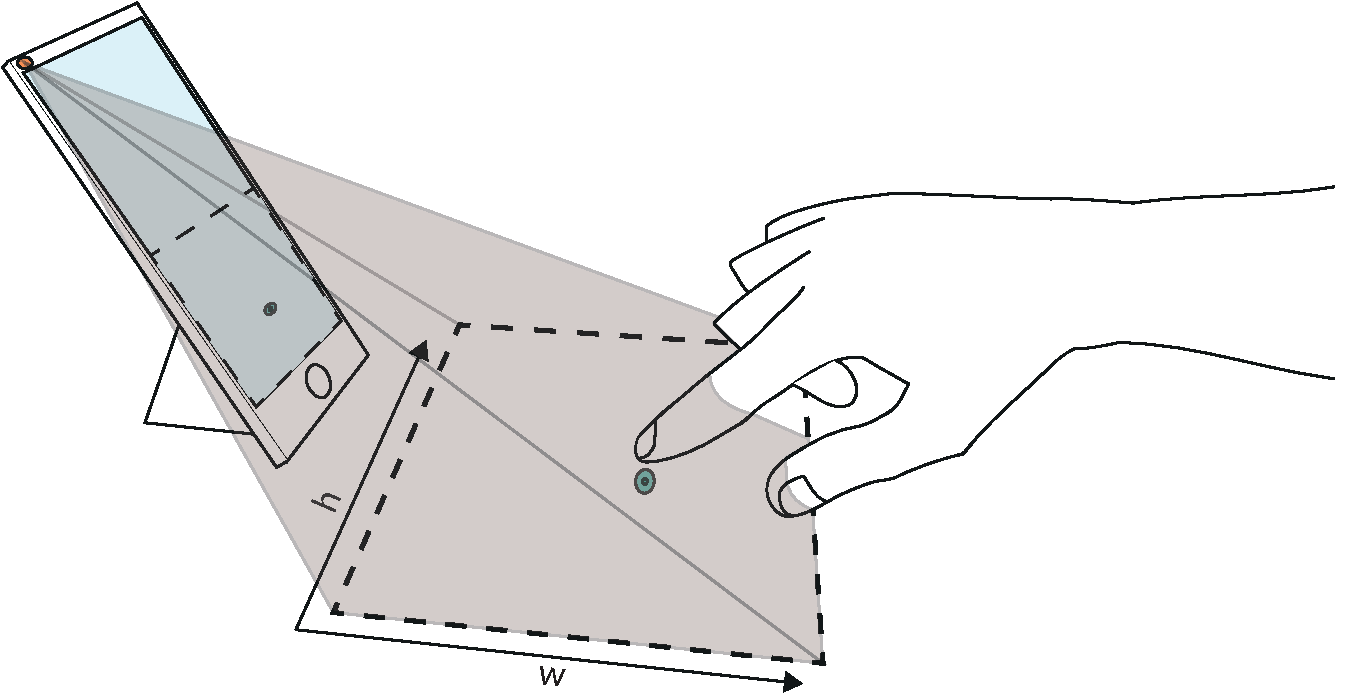
\includegraphics[width=\marginparwidth]{figures/banner.pdf}
        \caption{Potential interaction setup. A mobile device whose optical sensor creates an on-demand touch surface offers width and height as free parameters.}
        \label{fig:banner}
    \end{center}
\end{figure}
\begin{figure}
    \begin{center}
        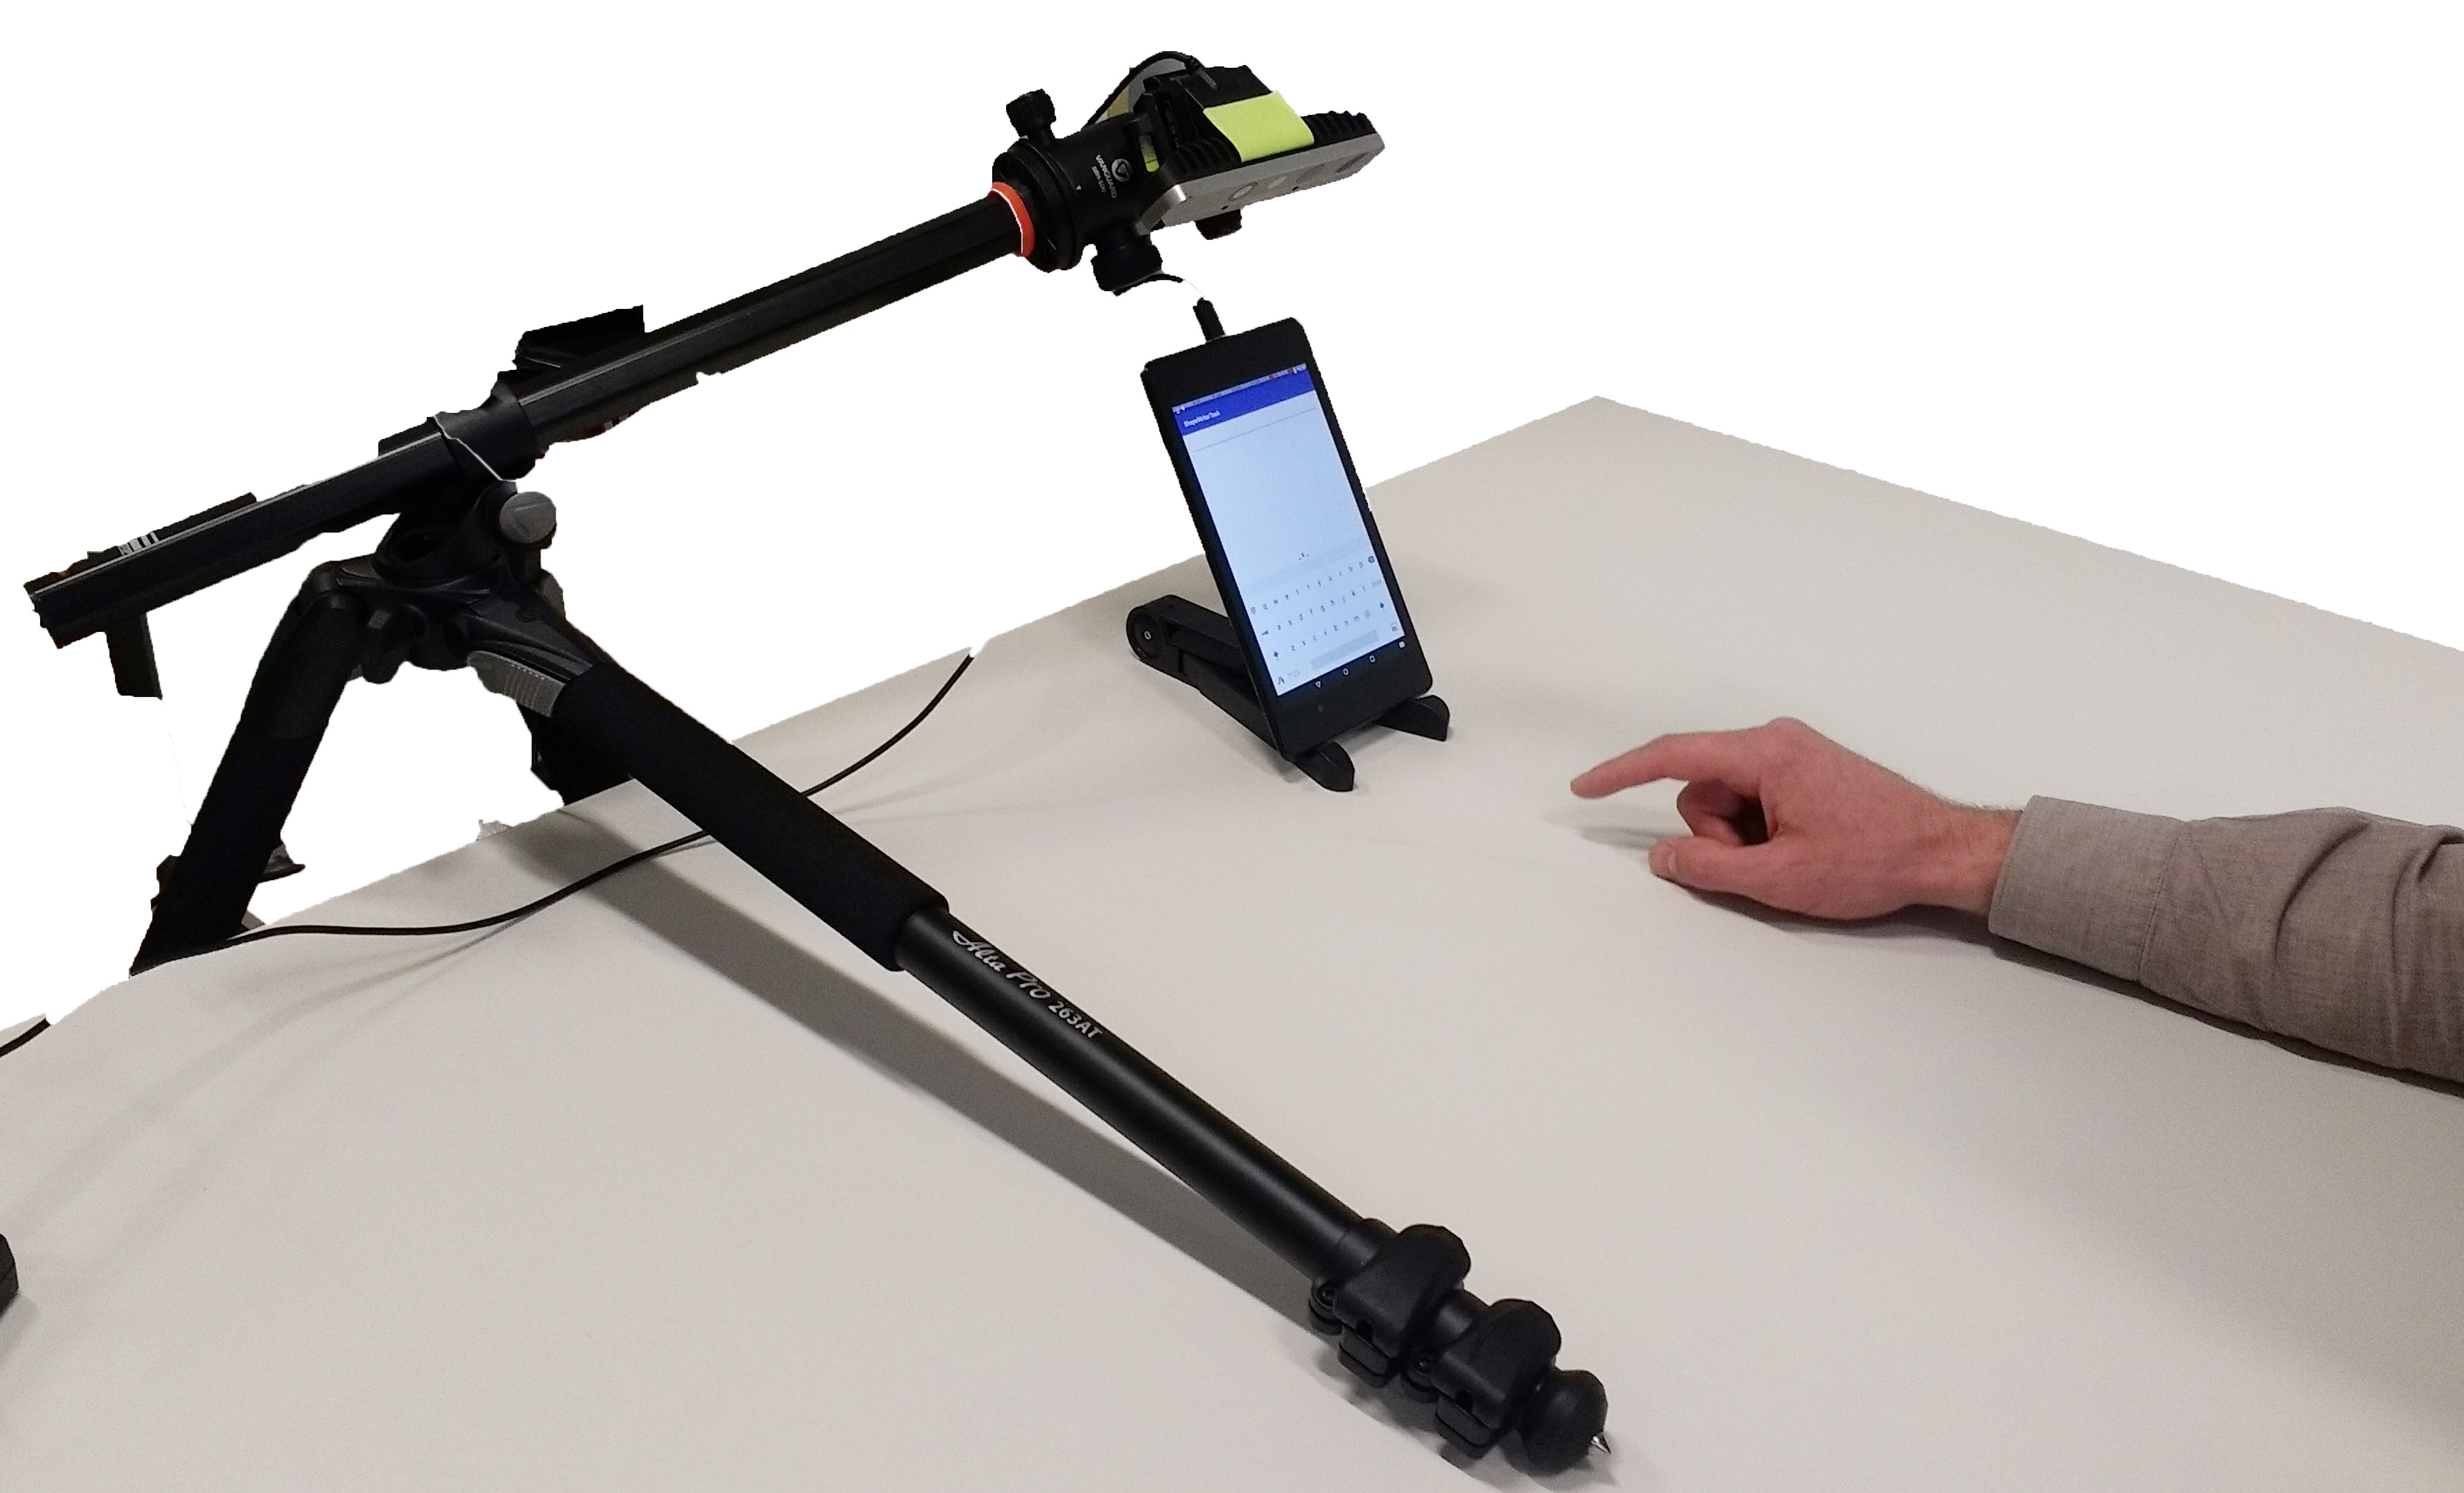
\includegraphics[width=\marginparwidth]{figures/system_insitu_0.jpg}
        \caption{Picture of the user study setup. A tablet device provides the audiovisual feedback while a depth camera mounted on a tripod creates a virtual touch input surface.}
        \label{fig:system_insitu_0}
    \end{center}
\end{figure}
}

% \textcolor{red}{potential for more space}

% \textcolor{red}{potential for more space}

In this context, the task of gesture typing~\cite{Kristensson2004} is interesting to research for the following reasons. Text-input remains a major activity~\cite{McGregor2014} on mobile device occupying up to 40\% of the user interaction time, the technique lends itself well to optical systems by limiting the requirement for repetitive target acquisition or touch classification, and little is known about the impact of input size (one of the free parameters of virtual surface) on writing performance.

This work specifically focus on two goals: to report on a supervised learning approach to the fingertip touch classification task and to study the influence of input space (size and aspect ratio) on gesture typing performance.
% \begin{itemize}
% \item to report on a supervised learning approach to the fingertip touch classification task.
% \item to study the influence of input space (size and aspect ratio) on gesture typing performance.
% \end{itemize}

% =============================================================================
\section{System overview}
% =============================================================================
The envisioned interaction scenario is shown in ~\autoref{fig:banner} with its implementation in \autoref{fig:system_insitu_0}. We use an Intel Realsense SR300 obliquely mounted on a tripod that overlooks the interaction surface. Finger detection and tracking is performed on a desktop computer. The system implements the 3 state button model, with its touch events sent to the Android tablet running a custom application overwriding its input event system. In addition, hover state is displayed as a red marker at the pointer’s position, touching is displayed through the Android debugging facility as a cross spanning the screen and continuous touch is displayed as a trace. An audio feedback is produced on each touch down event.

The pointer tracked by the system is defined as the point cloud closest to the camera in the depth direction ($y$ on ~\autoref{fig:pointcloud}); there is no explicit finger or hand modeling performed. Instead, the assumption is that the interacting finger is the furthest protruding object from the user.

The touch classification problem is usually solved via flood-filling~\cite{Harrison2011,Xiao2016}. However, it is well suited to a supervised learning approach provided availability of a training dataset. One of the authors video-taped 6 minutes of interactions, half touching and half hovering with some frames out of range while using the index, thumb and pinky at close and long range. From the fingertip pointcloud, we use the histogram of z-values as features (providing some orientation and shape invariance) and a neural network classifier. We tested the generalisation with different cross validation splits and obtained an averaged 0.96 AUC for the ROC, see~\autoref{fig:roc_auc}. The ROC curves led us to choose an operating point of 0.5 for the live system, which we trained on the whole dataset for 75 epochs.



% \begin{figure}
%   \centering
%   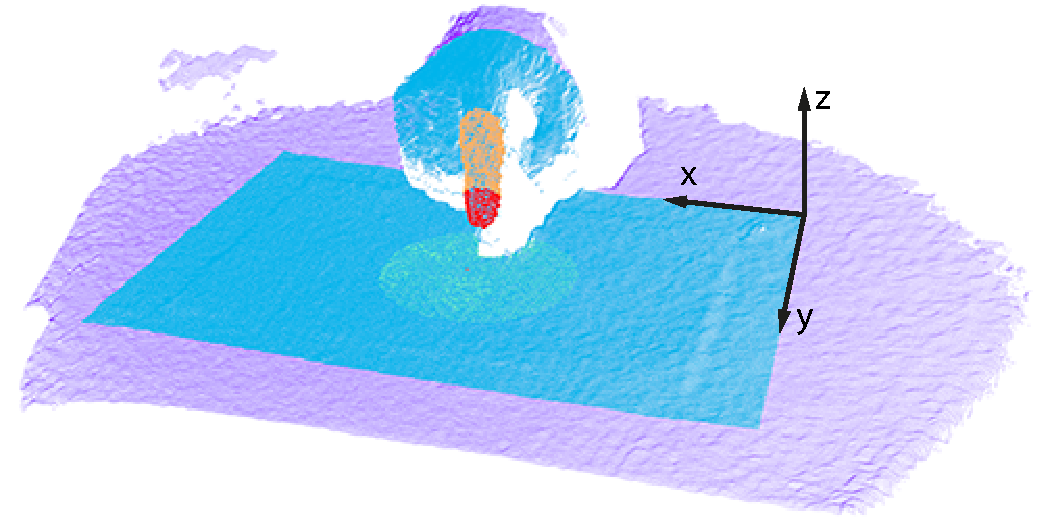
\includegraphics[width=\linewidth]{./figures/pointcloud.pdf}
%   \caption{Insert a caption below each figure.}
%   \label{fig:sample}
% \end{figure}

% =============================================================================
\section{User study}
% =============================================================================
We ran an experiment with two research goals in mind. First we wanted to evaluate the usability of our system, for this purpose we included a condition with an interaction directly on the tablet. Second, given the nature of the task and its inherent difficulty for novice users, we investigated the influence of the physical space on performance (Accot et al.~\cite{Accot2001} showed a U-shaped curve in performance). Our independent variable was thus the control surface dimensions, which is effectively changing the control-display gain defined by: $CD_{gain} = V_{display}/V_{control}$.

\marginpar{
\begin{figure}
    \centering
    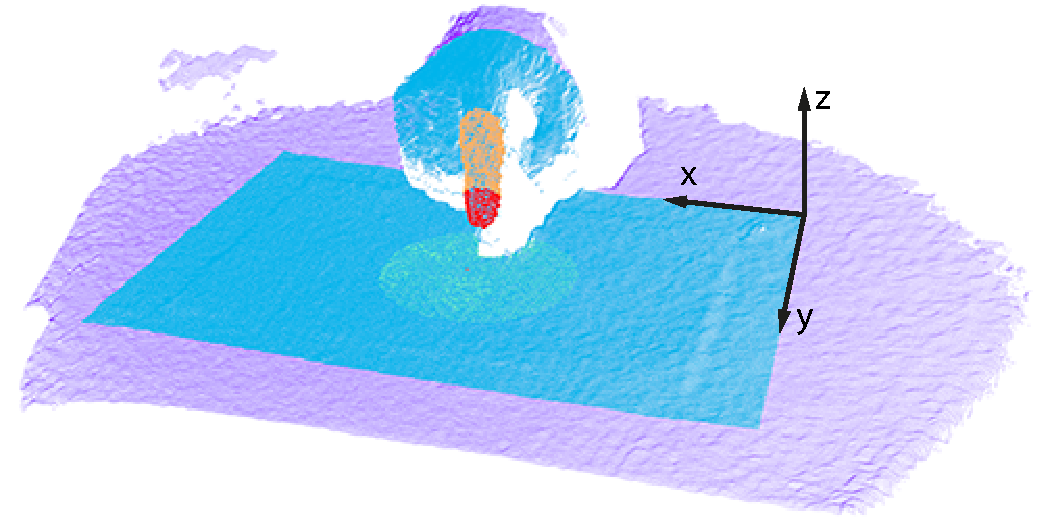
\includegraphics[width=\linewidth]{figures/pointcloud.pdf}
    \caption{Segmented sensor image with points within the interactive surface (blue), the ROI plane (cyan), the detected fingers (yellow) and the user pointer (red).}
    \label{fig:pointcloud}
\end{figure}

\begin{figure}
    \centering
    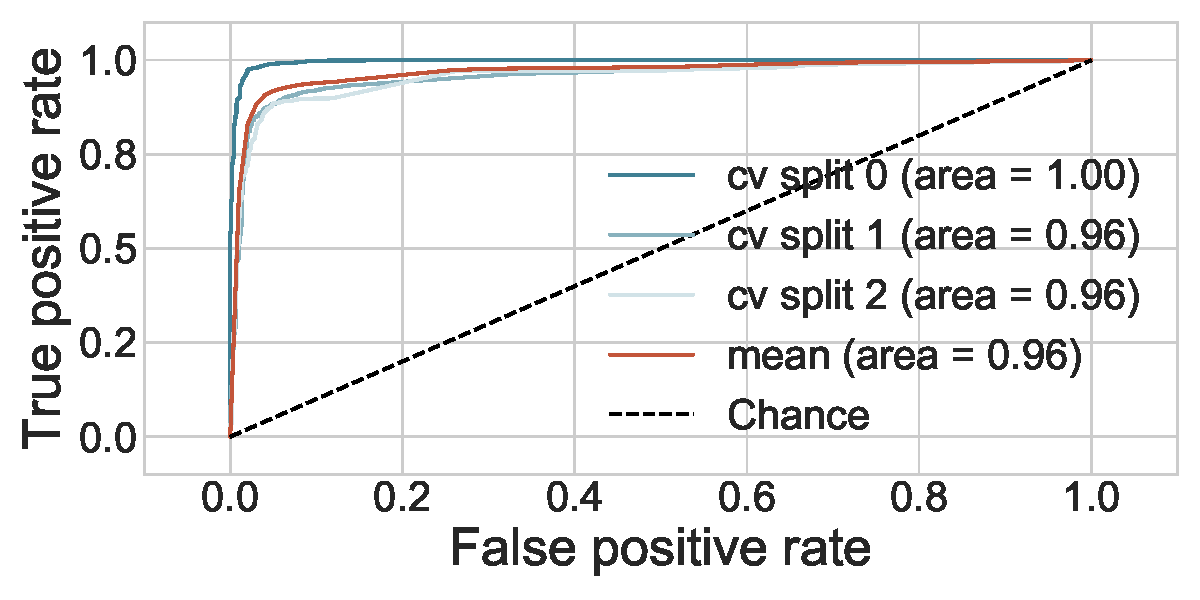
\includegraphics[width=\linewidth]{figures/roc_auc.pdf}
    \caption{Performance of the fingertip touch classification.}~\label{fig:roc_auc}
\end{figure}
}

We gathered 12 participants, all right handed, without requirement on gesture typing experience. A repeated measures within-subjects design was used. There were 3 conditions and 5 level combinations were evaluated, see \autoref{tab:cdt} for details. The presentation order of the 5 combinations was randomised and presented a uniform distribution across the participants. The task was to write 20 words per level (words taken at random from the most common english words with length between 2 and 5 letters) with maximum 7 attempt to complete 5 correct input for each word. The design of the task is similar to \cite{Quinn2016} and allows novice users to focus on the physical execution instead of the shape recollection, effectively emulating a proficient bahavior even for novice users. After each level, participants were offered to take a break before moving to the next one. Finally, participants were asked for their feedback using the NASA Task Load Index~\cite{Hart1988} (NASA-TLX) to assess the perceived workload of completed level.

\begin{table}
  \centering
  \begin{tabular}{l l | r r r r r}
    \smit{LEVEL} & \smit{DEVICE} & \smit{width} & \smit{height} & \smit{area}& \smit{ratio} & \smit{$CD_{gain}$} \\
    % \midrule
    \hline
    \cdt{OP1} & \cdt{optical} & 9.4 & 4.7 & 44.2 & 2 & 1 \\
    \cdt{OP2} & \cdt{optical} & 18.8 & 9.4 & 176.7 & 2 & 1/2 \\
    \cdt{OL2} & \cdt{optical} & 25.6 & 6.9 & 176.6 & 3.7 & 1/1.7 \\
    \cdt{OP4} & \cdt{optical} & 37.7 & 18.9 & 712.5 & 2 & 1/4 \\
    % \midrule
    \hline
    \cdt{tp1} & \cdt{tablet} & 9.4 & 4.7 & 44.2 & 2 & 1 \\
  \end{tabular}
  \caption{Design of the experiment. Level name, device type, dimensions (in $cm$), area (in $cm^2$), ratio and control/display gain for all 5 combinations used in the experiment.}~\label{tab:cdt}
\end{table}

The experimental design was thus: 12 participants $\times$ 5 \cdt{level} $\times$ 20 \cdt{word} = 1200 trials. For each trial, we had 5 to 7 attemps depending on the error rate, which means a total of 6,000 to 8,400 total samples. After the experiment, we actually recorded 6963 samples.

% =============================================================================
\section{Result}
% =============================================================================
The dependent variables are the success rate, the time taken per trial and the trace data when available. This allowed us to compute the dependent measure error rate defined as the percentage of unsucessful attempts as well as the text entry rate measured in Words Per Minute (WPM), as in [3], according to the formula\footnote{$WPM = |T|/s \times 60/5$ where $|T|$ is the length of the transcribed string, s is time in seconds}.

We found one input word (\cdt{lay}) presented some very unusual behavior. Entry rates had an error rate at $89.5\%$ while the WORD mean is $20.1\%$ and no other word had an error rate higher than $30\%$. The reason is that the recogniser promotes words of higher prior probability in the language model, in this case “Larry”, “last” or “Katy” - highlight the limitations of pure gesture typing interaction.

A statistical analysis showed a significant main effect of DEVICE ($F_{1,11} = 37.77, p < 0.0001$) on error rate with mean value for TP1 and OP1 equal to respectively 6.2\% and 26.1\%, see Figure 4.a. A statistical analysis also showed a significant main effect of SIZE ($F_{2,22} = 10.99, p < 0.001$) on the error rate. Finally, an ANOVA on TP1, OP2, OP4 and OL2 did not show a significant main effect (p = 0.11) even though OPTICAL is in average higher than TABLET. In other words, among all levels of the experiment, only OP1 shows a significant higher error rate.

A statistical analysis showed a significant main effect of DEVICE ($F_{1,11} = 90.15, p < 0.0001$) on input rate with mean values for TP1 and OP1 equal to respectively 29.2 WPM and 13.7 WPM. We also looked at pair-wise comparison2 for OP-TICAL and could not find a statistical difference in the mean input rate. The input rate achieved by the participants in TP1 is in-line with what can be expected from novice users after the time of the experiments~\cite{Kristensson2004}. The averaged 54\% lower input rate in OPTICAL should be compared with other simi- lar results, as~\cite{Markussen2014} with 57\% after 10 sessions, that compare direct and indirect input modality for mid-air gesture typing.


The participants were capable of moving their hand with great variability when it comes to speed.

The Nasa TLX reported high stress on big surfaces, and high stress on the very small surface. As a results, the optimal size is in the middle.

% \begin{figure}
% \centering     %%% not \center
% \subfigure[]{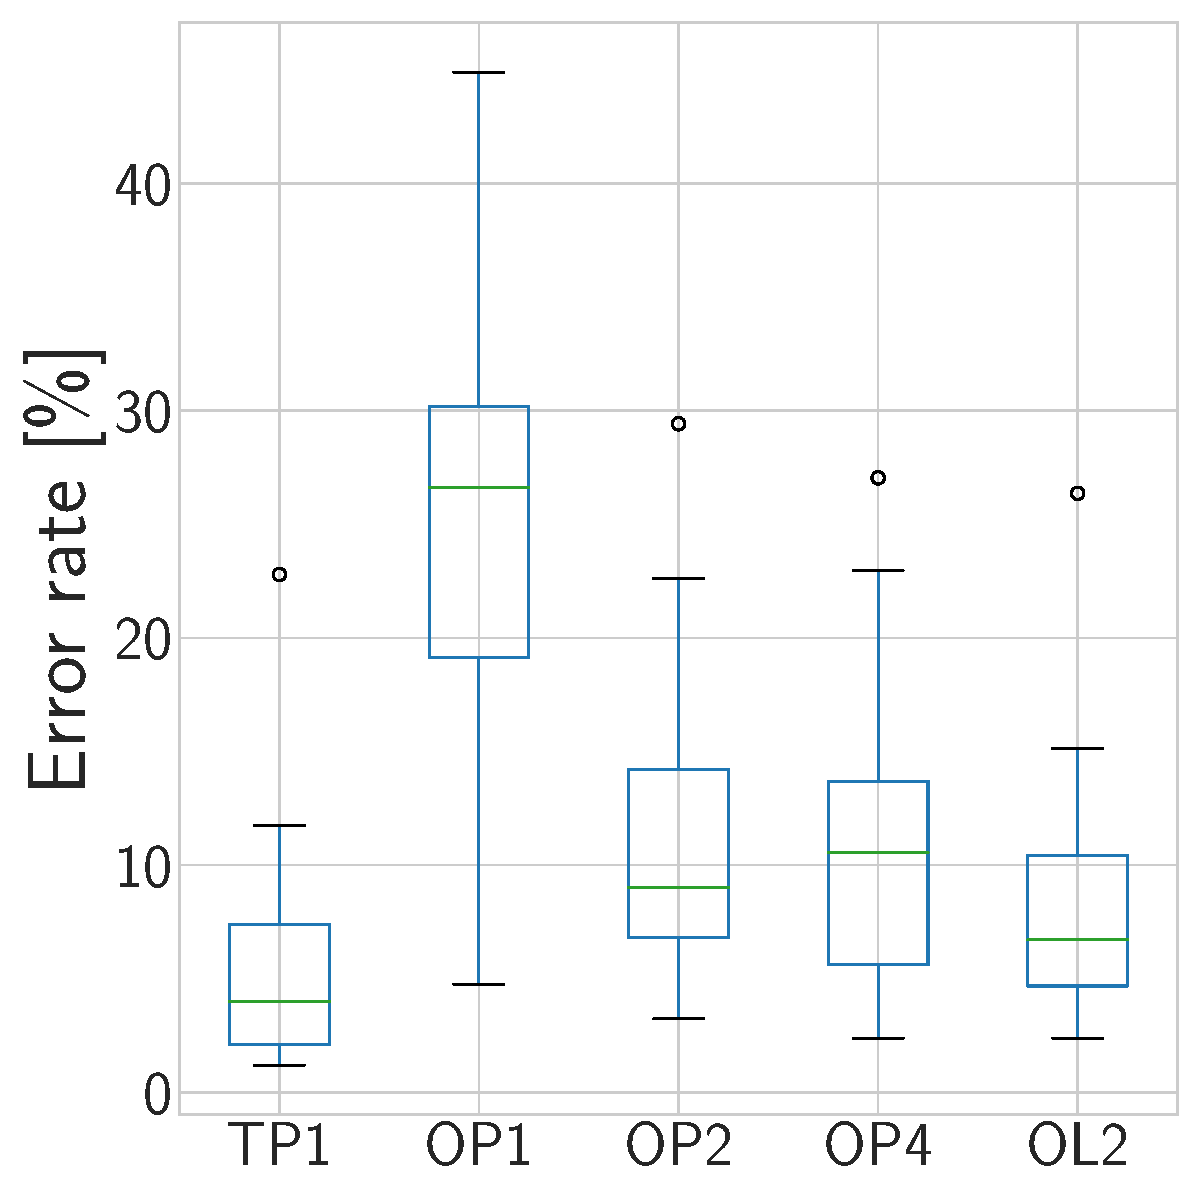
\includegraphics[width=0.49\linewidth]{figures/err_DEVICE_SHAPE.pdf}}
% \subfigure[]{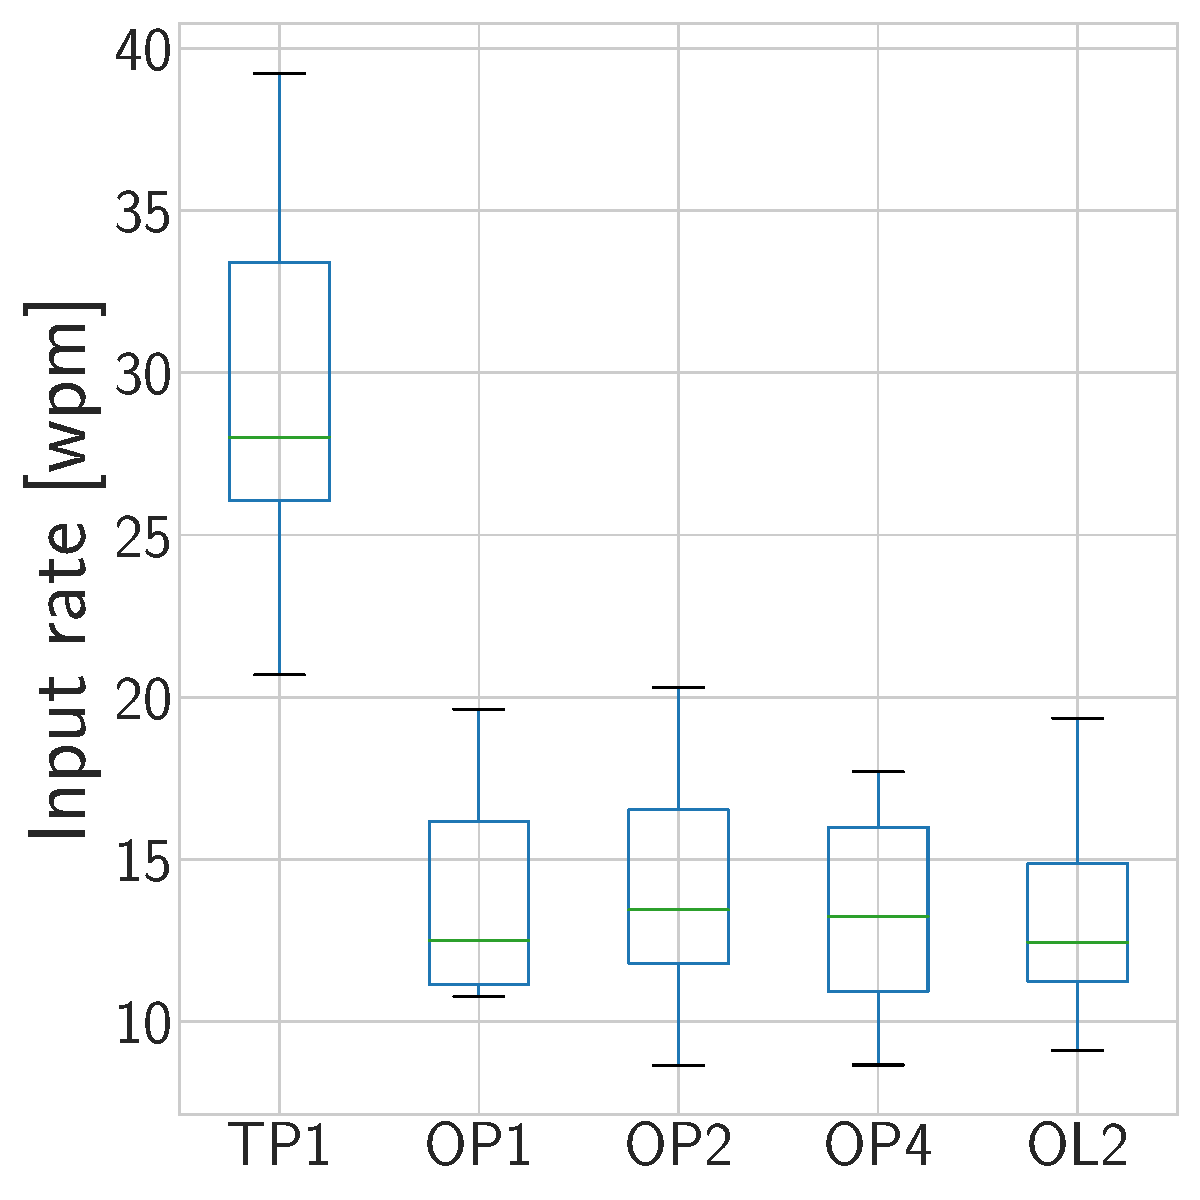
\includegraphics[width=0.49\linewidth]{figures/wpm_DEVICE_SHAPE.pdf}}
% \caption{Effect of levels on error rate (a) and input rate (b).}~\label{fig:effect_shape}
% \end{figure}

% =============================================================================
\section{Conclusion and Future work}
% =============================================================================

\marginpar{
\begin{figure}
    \centering
    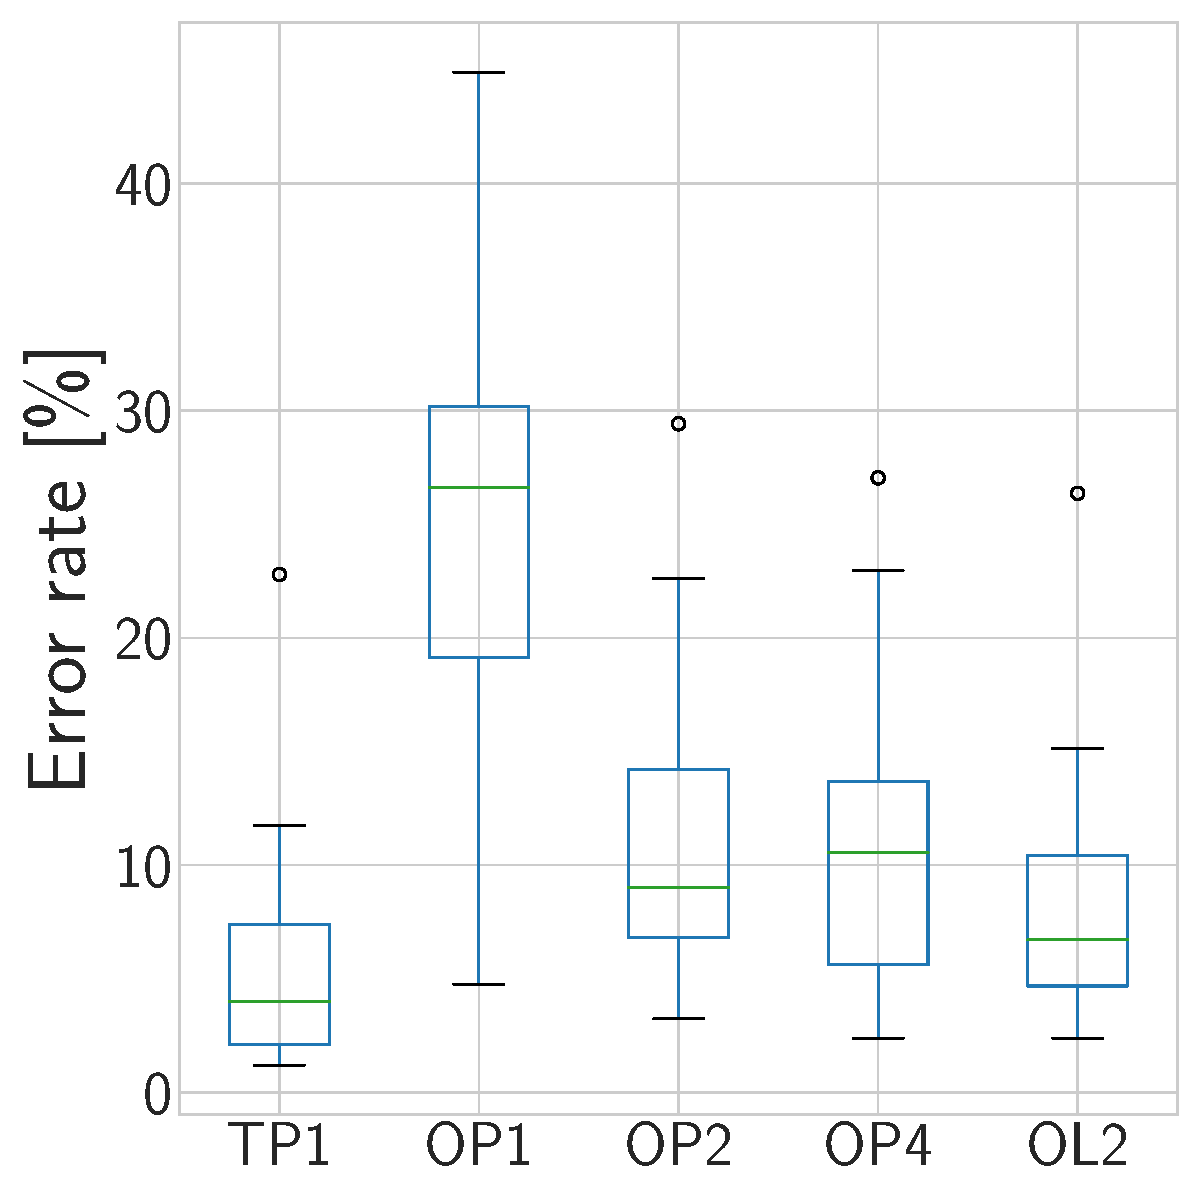
\includegraphics[width=\linewidth]{figures/err_DEVICE_SHAPE.pdf}
    \caption{Effect of levels on error rate.}
    \label{fig:err_DEVICE_SHAPE}
\end{figure}

\begin{figure}
    \centering
    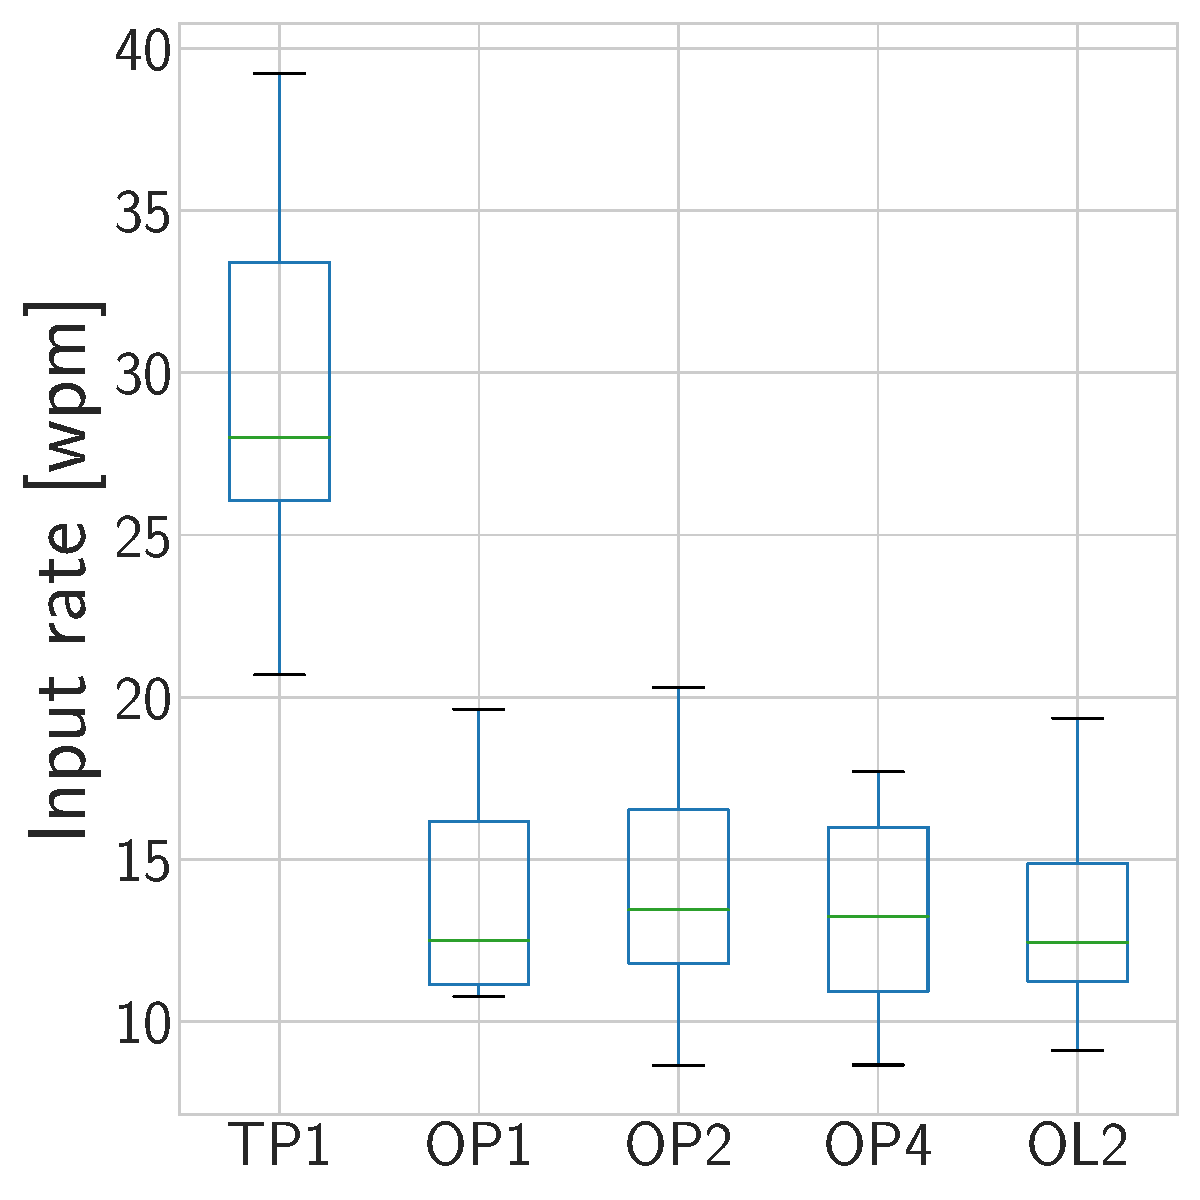
\includegraphics[width=\linewidth]{figures/wpm_DEVICE_SHAPE.pdf}
    \caption{Effect of levels on input rate.}
    \label{fig:wpm_DEVICE_SHAPE}
\end{figure}
}
The user study showed that the users hit the accuracy ceiling when using a small surface. It also showed that the task behave according to Fitts law. The users seem to be limited by their ability to drive an indirect pointer rather than performing the difficulty of the task itself.

These encouraging results open the way to testing the system with patients with spinal cord injury. More so, due to recent advance in hand pose recognition, the reality of interacting via touch through vision based system should be investigated further.

% \section{Acknowledgements}
% We would like to thank the EU Moregrasp project for funding the research, as well as the patients in the spinal unit in Heidelberg for providing early feedback about the interaction technique.


\newpage

\balance
\bibliographystyle{acm-sigchi}
\bibliography{collection}

\end{document}